\zerar
\chapter{Resultados}
\label{cap:resultados}

Em nosso estudo, utilizamos os pacotes de otimização GLPK (GNU Linear Programming Kit) e Cplex da
IBM. Os resultados finais, entretanto, são baseados apenas na utilização da ferramenta Cplex, uma
vez que a mesma provou ser mais eficiente. Além disso, o otimizador Cplex pôde ser utilizado
diretamente a partir de nosso código, alimentando o modelo gerado através da API Java fornecida pela
IBM. Por outro lado, como o GLPK não fornece API apropriada, sua utilização se limitou a geração do
modelo em arquivo (formato mps) e posterior execução do otimizador em um processo separado, sendo
necessário realizer um {\it parsing} no arquivo de saída gerado para obtenção dos resultados.

Restringimos o nosso estudo de escalonamento à resolução do problema de determinação de viagens.
Implementamos os métodos de solução do PDV descritos na Seção~\ref{sec:metodos}. Os parâmetros 
utilizados, que garantem a legalidade das viagens geradas, são apresentados na 
Tabela~\ref{tab:parametros} e baseiam-se na legislação brasileira para aviação comercial regular. 

Todos os testes foram realizados em um computador utilizando um processador Intel Core~i3 64~bits, 
com 4~Gb de memória RAM, rodando o sistema operacional MacOS~10.6. Toda a implementação foi escrita 
em Java (JDK~1.6.33).

\begin{table}
	\begin{center}
		\begin{tabular}{|l|l|l|}
			\hline 
			\bf Parâmetro & \bf Descrição & \bf Valor \\
			\hline \hline 
			\verb|MAX_LEGS| & Máximo de pernas por jornada & 5 \\ \hline
			\verb|MAX_FLIGHT_TIME| & Total máximo de voo por jornada & 9,5 h \\ \hline
			\verb|MAX_DUTY_TIME| & Duração máxima de uma jornada & 11,5 h \\ \hline
			\verb|MIN_SIT_TIME| & Tempo mínimo de conexão & 30 min \\ \hline
			\verb|MAX_SIT_TIME| & Tempo máximo de conexão & 120 min \\ \hline
			\verb|BRIEFING_TIME| & Tempo para o {\it briefing} & 0 min \\ \hline
			\verb|DEBRIEFING_TIME| & Tempo para o {\it debriefing} & 0 min \\ \hline
			\verb|MIN_REST_TIME| & Tempo mínimo de repouso & 12 h \\ \hline
			\verb|MAX_REST_TIME| & Tempo máximo de repouso & 36 h \\ \hline
			\verb|MAX_DUTIES| & Máximo de jornadas por viagem & 2, 3 ou 4 \\ \hline
			\end{tabular} 
			\caption{Parâmetros utilizados na geração das viagens.}
			\label{tab:parametros}
	\end{center}
\end{table}

%%%%%%%%%%%%%%%%%%%%%%%%%%%%%%%%%%%%%%%%%%%%%%%%%%%%%%%%%%%%%%%%%%%%%%%%%%%%%%%%%%%%%%%%%%%%%%%%%%%%

\section{Análise Preliminar}
\label{sec:preliminar}

O objetivo desta análise preliminar foi definir o limite de utilização do procedimento de geração
de viagens e do otimizador na resolução exata do modelo {\it set partition} (\ref{eq:sppv}).
Com essa finalidade, construímos alguns gráficos que relacionam o tempo de geração e otimiazação 
utilizado em nossa implementação, em função do número de etapas dadas como entrada do problema.

Para estudar a influência do número de pernas isoladamente, restringimos a entrada apenas para um
conjunto de voos entre duas localidades, São Paulo (CGH) e Rio de Janeiro (SDU), considerando os
trechos diárias oferecidos na ponte-aérea pela companhia aérea Gol. Um total de 62 pernas 
(31 de CGH para SDU e 31 de SDU para CGH) representam a instância global de entrada.

Vale observar que o caso da ponte-aérea é um pouco atípico no sentido de que representa um malha 
muito densa de voos: muitas etapas são oferecidas de ida e volta num curto intervalo de tempo, 
criando muitas conexões legais (arcos) entre os nós da rede de voos gerada. Com isso, o número
de viagens dado pela procedimento de busca no grafo explode rapidamente.

O gráfico da Figura~\ref{fig:pairings} mostra o número de viagens geradas em função do número de
etapas na ponte-aérea. As viagens foram geradas para a base CGH. São apresentadas três curvas, uma
para cada valor do parâmetro \verb|MAX_DUTIES| (2, 3 e 4). Observe a escala logarítmica do eixo
vertical. O comportamento praticamente linear das curvas indica um crescimento exponencial do número
de viagens que podem ser geradas. Observe ainda que a taxa de crescimento é maior quanto maior o
número máximo de jornadas permitidas, já que nesse caso permite-se um número muito maior de
combinações. Para \verb|MAX_DUTIES| = 4, encontrou-se um número da ordem de $10^8$ viagens com
apenas 36 pernas.

\begin{figure}[htp]
	\begin{center}
		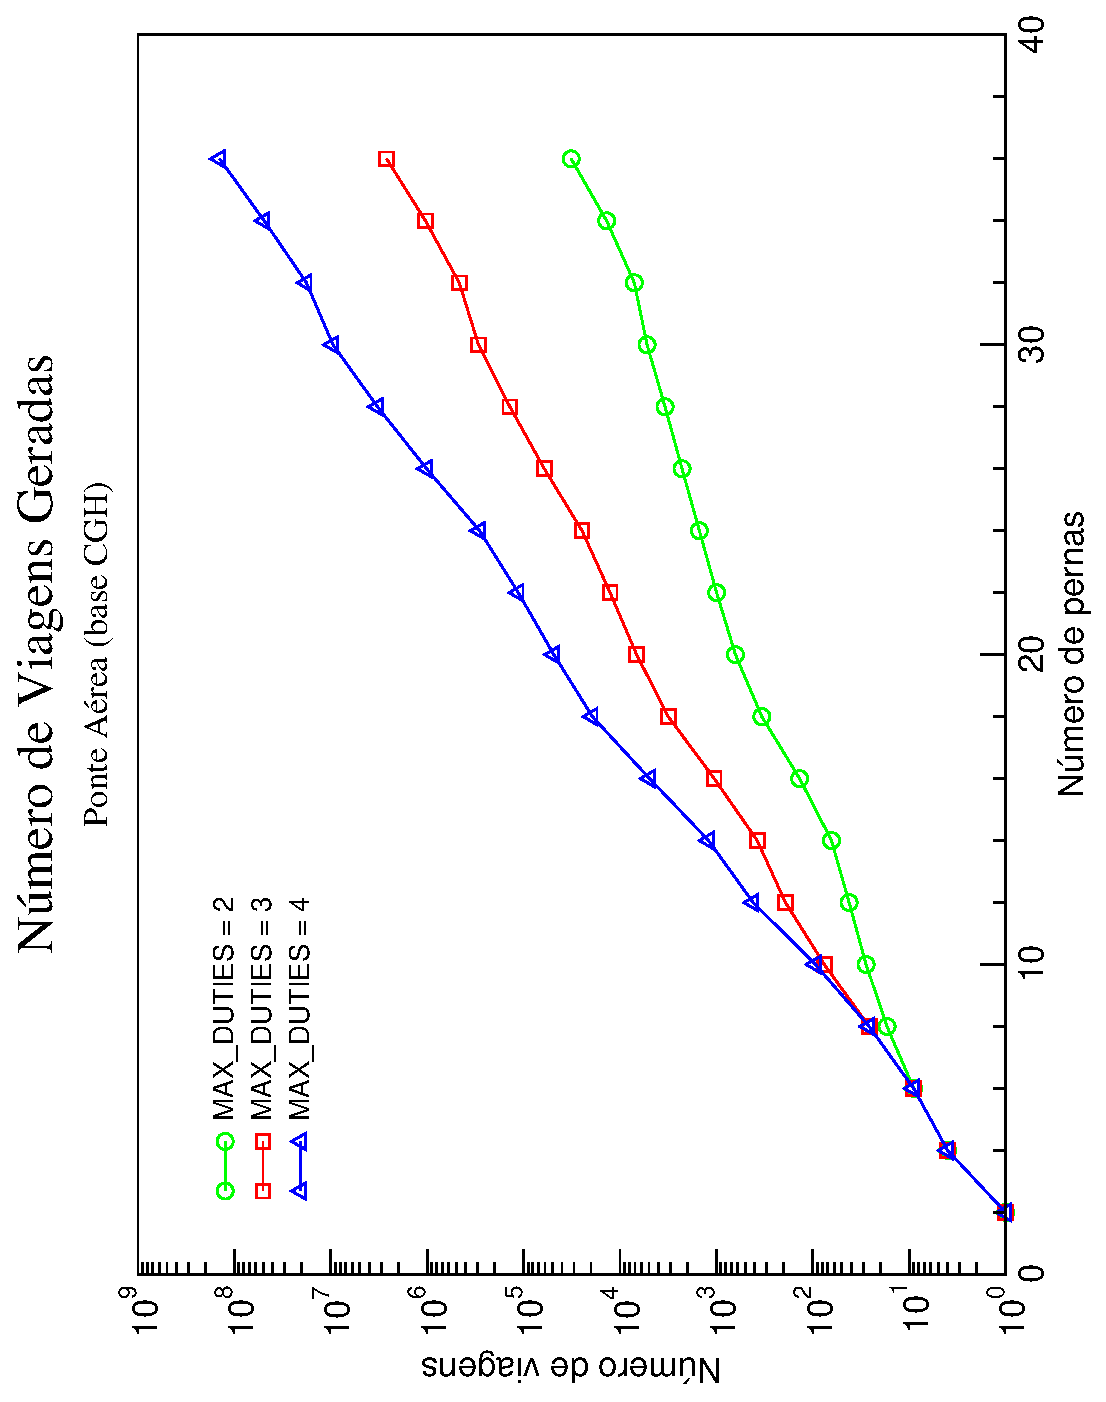
\includegraphics[scale=0.45,angle=-90]{fig/number_of_pairings.eps}
		\caption{Número de viagens geradas em função do número de pernas utilizadas na construção da
		rede de voos.}
		\label{fig:pairings}
	\end{center}
\end{figure}

O consumo de tempo gasto pelo algoritmo de busca em profundidade também foi medido em função do 
número de pernas. Os resultados são apresentados na Figura~\ref{fig:generation}. O comportamento das
curvas indicam também um crescimento exponencial do tempo gasto pelo algoritmo, ainda que ele seja
executado de forma rápida (para \verb|MAX_DUTIES| = 4, encontrou-se um tempos da ordem de $10^4$~ms 
para 36 pernas).

\begin{figure}[htb]
	\begin{center}
		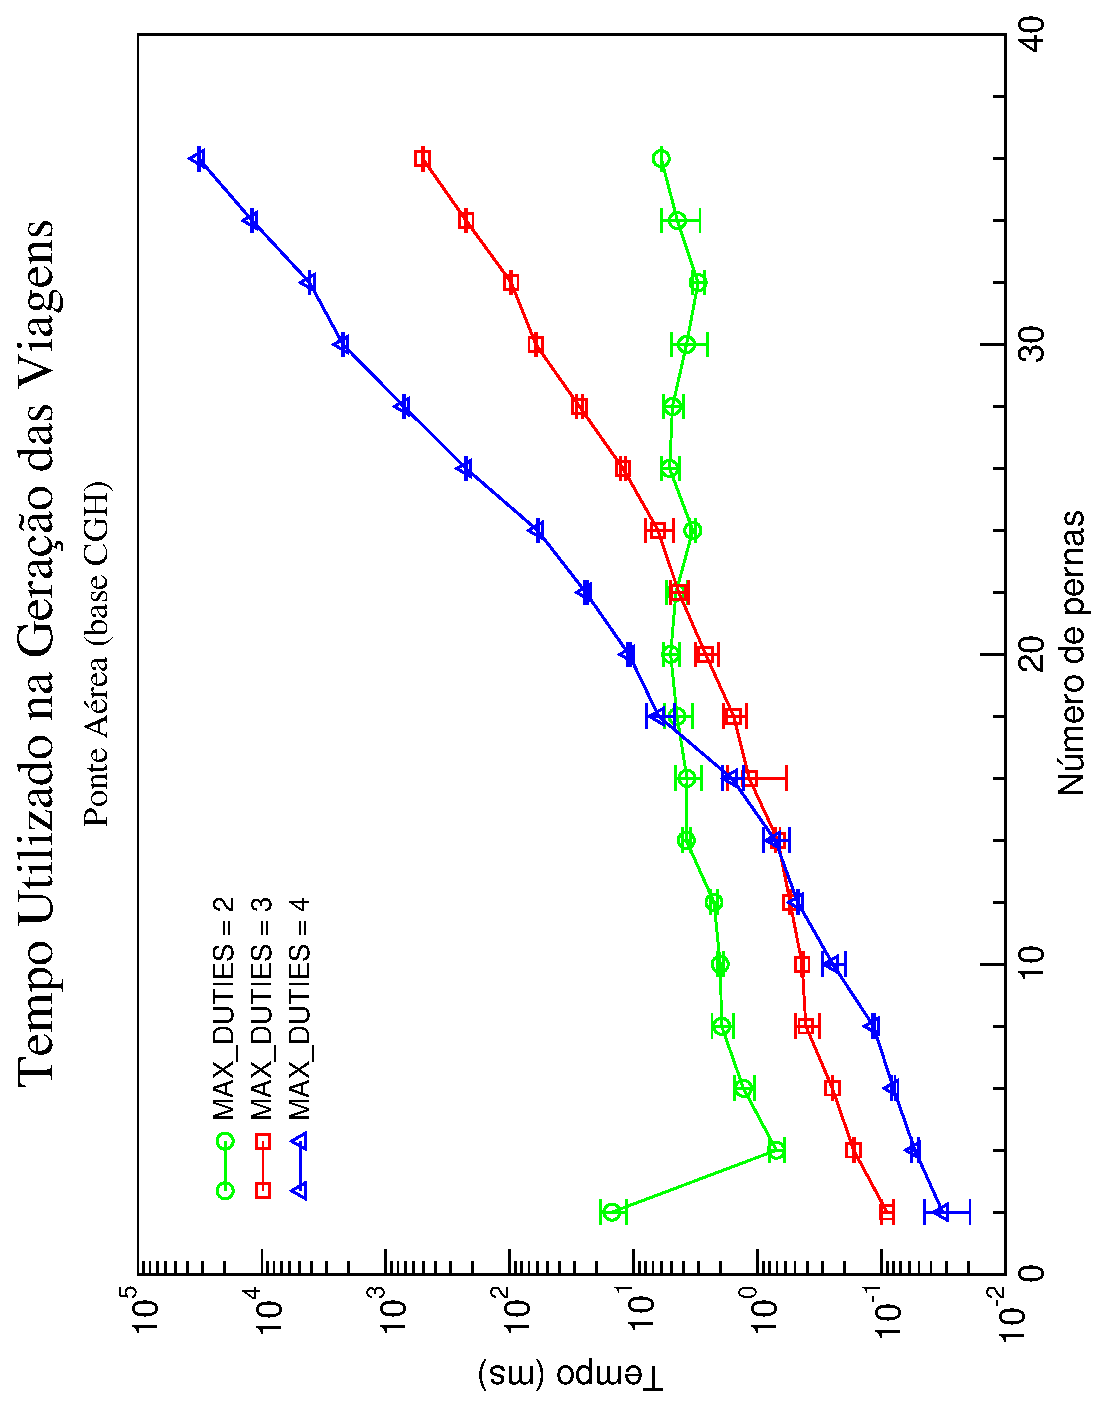
\includegraphics[scale=0.45,angle=-90]{fig/generation_time.eps}
		\caption{Tempo gasto na geração das viagens em função do número de pernas utilizadas na 
		construção da rede de voos. São apresentados valor médio $\pm$ desvio-padrão, considerando 5 
		medidas para cada ponto. O primeiro ponto da curva verde encontra-se um pouco fora provavelmente
		devido a algum transiente da máquina, visto que ele foi o primeiro a ser processado.}
		\label{fig:generation}
	\end{center}
\end{figure}

O tempo gasto pelo otimizador GLPK para resolver o modelo proposto é apresentado no gráfico da 
Figura~\ref{fig:glpk}. Mais uma vez, observa-se um crescimento exponencial muito forte (note a 
escala logarítmica do eixo vertical) em função do número de etapas considerado. A 
Figura~\ref{fig:cplex} mostra os resultados obtidos para o otimizador Cplex. 

\begin{figure}[htb]
	\begin{center}
		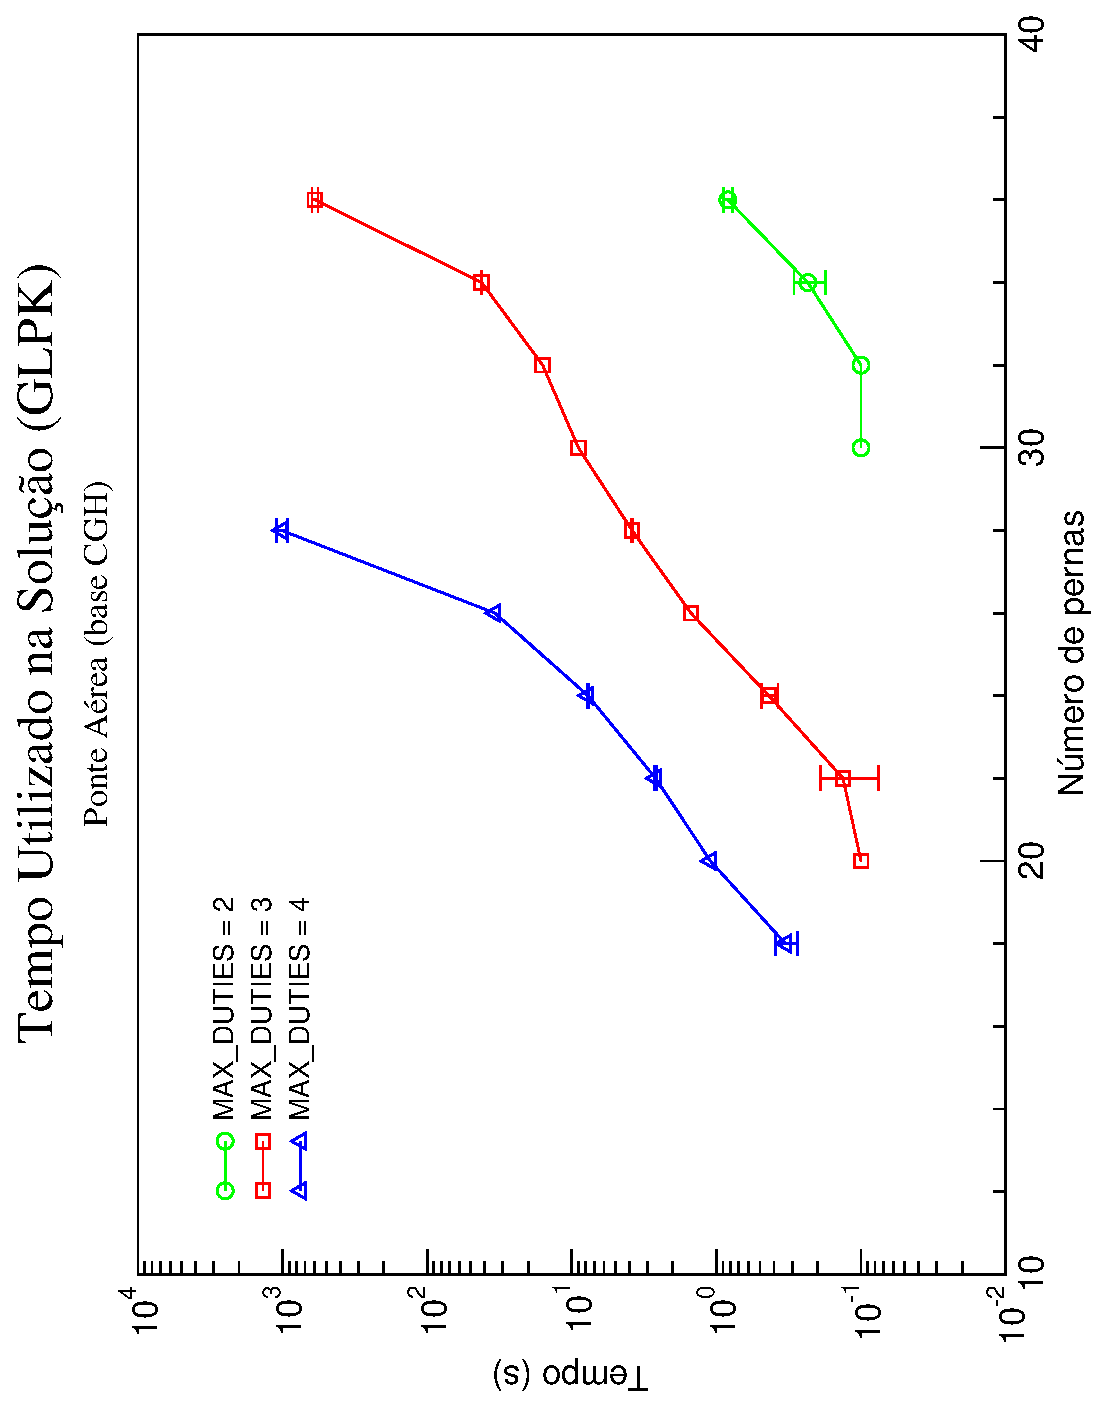
\includegraphics[scale=0.45,angle=-90]{fig/glpk_solution_time.eps}
		\caption{Tempo utilizado pelo otimizador GLPK na obtenção de uma solução inteira, em função do 
		número de etapas. São apresentados valor médio $\pm$ desvio-padrão, considerando 3 medidas para 
		cada ponto. Valores medidos com tempo de execução de 0,0~s não são apresentados (número pequeno 
		de pernas). Os últimos pontos da curva azul não puderam ser estimados, mesmo após algumas horas 
		de processamento.}
		\label{fig:glpk}
	\end{center}
\end{figure}

\begin{figure}[htb]
	\begin{center}
		\includegraphics[scale=0.45,angle=0]{fig/cplex_solution_time.eps}
		\caption{Resultados obtidos para o otimizador Cplex. Valem as mesmas observações feitas na 
		legenda da Figura~\ref{fig:glpk}.}
		\label{fig:cplex}
	\end{center}
\end{figure}

%%%%%%%%%%%%%%%%%%%%%%%%%%%%%%%%%%%%%%%%%%%%%%%%%%%%%%%%%%%%%%%%%%%%%%%%%%%%%%%%%%%%%%%%%%%%%%%%%%%%

\section{Instâncias Estudadas}
\label{sec:instancias}

%%%%%%%%%%%%%%%%%%%%%%%%%%%%%%%%%%%%%%%%%%%%%%%%%%%%%%%%%%%%%%%%%%%%%%%%%%%%%%%%%%%%%%%%%%%%%%%%%%%%

\section{Soluções Exatos}
\label{sec:solucoes_exatas}

Apenas três instâncias (pequenas) puderam ser resolvidas exatamente pela solução do modelo {\it set
partition} (\ref{eq:sppv}), com um tempo de processamento pequeno. A descrição das instâncias é
apresentada na Tabela~\ref{tab:instancias}, as quais foram extraídas de dados reais fornecidos por
companhias aéreas brasileiras. Na tabela são indicados o nome da instância, a companhia a qual
pertence, a frota de aeronaves (ou parte dela) a que se refere, as bases domiciliares dos
tripulantes, o número de etapas e o número de trilhos. O trilho identifica o conjunto de etapas que
uma determinada aeronave da frota deve executar diariamente. No caso de uma frota com $k$ aeronaves,
deverão ser fornecidos $k$ trilhos distintos.

\begin{table}[htb]
	\begin{center} 
		\begin{tabular}{|l|l|l|l|l|l|}
			\hline 
			{\bf Instância} & {\bf Cia} & {\bf Frota} & {\bf Bases} & {\bf Etapas} & {\bf Trilhos} \\ 
			\hline \hline
			73H\_26 & Gol & 737-800 & GRU & 26 & 5 \\ 
			738\_48 & WebJet & 737-800 & GRU GIG & 48 & 7 \\ 
			733\_92 & WebJet & 737-300 & GRU GIG POA & 92 & 12 \\ \hline
		\end{tabular}
		\caption{Caracterização das instâncias resolvidas exatamente através dos modelos 
		{\it set partition} e {\it set cover}. GRU = São Paulo, GIG = Rio de Janeiro e 
		POA = Porto Alegre.}
		\label{tab:instancias}
	\end{center}
\end{table}

Na resolução dos problemas, foram utilizados os parâmetros da Tabela~\ref{tab:parametros}. Além
disso, limitou-se a 1 o número máximo de trocas de aeronaves por jornada. Com isso, forçamos a
tripulação acompanhar, na medida do possível, o trilho percorrido pela aeronave, reduzindo a
possibilidade de conexões em cada localidade. Naturalmente os tempos de conexão serão reduzidos,
tornando as viagens geradas mais baratas e diminuindo o número total de variáveis geradas. Além
disso, esse procedimento torna a solução mais robusta, uma vez que o atraso de uma aeronave não
acarretará atraso na saída de outro voo que dependa daquela aeronave na troca.

O custo de uma viagem foi calculado como sendo o tempo ``ocioso'' relativo no qual o tripulante está 
trabalhando mas não está voando, ou seja, pela diferença entre o tempo total de uma viagem, menos o 
tempo total de voo efetuado, descontando ainda os tempos mínimos regulamentares de conexão entre 
pernas e de descanso entre jornadas, dividido pelo tempo total de voo. Esse custo avalia de forma 
relativa a produtividade de uma viagem, o qual deve ser minimizado na solução final.

Os resultados obtidos são apresentados e resumidos na Tabela~\ref{tab:resultados}. Nela são 
indicadas a instância resolvida, o número total de variáveis geradas, o número de viagens na 
solução, o custo da solução e o tempo de processamento do otimizador (Cplex).

\begin{table}[htb]
	\begin{center} 
		\begin{tabular}{|c|c|c|c|c|}
			\hline 
			{\bf Instância} & {\bf Variáveis} & {\bf Viagens} & {\bf Custo} & {\bf Tempo (s)} \\ 
			\hline \hline
			73H\_26 & 180 & 6 & 6,952 & $< 1$ \\ 
			738\_48 & 66411 & 6 & 6,436 & 3,75 \\
			733\_92 & 1023818 & 11 & 6,942 & 170,86 \\ \hline
		\end{tabular}
		\caption{Resultados obtidos na geração e otimização de viagens para as instâncias consideradas.}
		\label{tab:resultados}
	\end{center}
\end{table}

As mesmas instâncias 73H\_26, 738\_48, 733\_92 também foram resolvidas utilizando o modelo 
{\it set cover}, o qual admite a existência de {\it deadheading}. Os resultados obtidos foram 
idênticos aos listados na Tabela~\ref{tab:resultados}. Em particular, todas as variáveis 
artificiais $y_i$ receberam valor zero na solução final, indicando a não necessidade de 
{\it deadheading}.

%%%%%%%%%%%%%%%%%%%%%%%%%%%%%%%%%%%%%%%%%%%%%%%%%%%%%%%%%%%%%%%%%%%%%%%%%%%%%%%%%%%%%%%%%%%%%%%%%%%%

\section{Um Resultado Explícito}
\label{sec:resultado_explicito}

Para tornar mais concreto a entrada e a saída do problema, apresentamos na Tabela~\ref{tab:73H_26} o
conjunto de etapas referentes a instância 73H\_26\footnote{Não há problema de confidencialidade nos
dados apresentados.}. A mesma representa 26 trechos oferecidos diariamente pela companhia aérea Gol
para uma frota especial de 5 aeronaves B737-800. Para cada etapa são fornecidos o seu número,
aeroporto de origem, aeroporto de destino, horário local de decolagem (DEP) e horário local de pouso
(ARR) e o trilho correspondente.

Na Tabela~\ref{tab:pairings} listamos as 6 viagens geradas como solução do problema de otimização.
Cada etapa na tabela apresenta o número do voo, origem e destino, horário local de decolagem e 
pouso, e o trilho executado. O custo final resultante foi de 6,952, para um total de 180 variáveis 
geradas, considerando a base GRU (São Paulo). Observe a presença de uma viagem bate-volta (4),
bem como uma viagem de 3 dias de duração (5).

\begin{table}[!htb]
	\begin{center}
		\begin{tabular}{|cccccc|}
			\hline 
			{\bf Número} & {\bf Origem} & {\bf Destido} & {\bf DEP} & {\bf ARR} & {\bf Trilho} \\
			\hline \hline
			7625 & GRU &	GIG	 &  07:00	 &  08:00  & 1 \\
			7622 & GIG &	GRU	 &  09:00	 &  09:55	 & 1 \\
			7622 & GRU &	CCS	 &  11:00	 &  15:30	 & 1 \\
			7622 & CCS &	AUA	 &  16:10	 &  17:55	 & 1 \\
			7623 & AUA &	CCS	 &  21:20	 &  22:05	 & 1 \\
			7623 & CCS &	GRU	 &  22:45	 &  06:00	 & 1 \\
			1841 & CWB &	GRU	 &  07:52	 &  08:55	 & 2 \\
			1902 & GRU &	NAT	 &  11:00	 &  14:20	 & 2 \\
			1903 & NAT &	GRU	 &  15:30	 &  19:10	 & 2 \\
			1704 & GRU &	MAO	 &  21:15	 &  00:10	 & 2 \\
			1798 & GRU &	REC	 &  08:05	 &  11:21	 & 3 \\
			1149 & REC &	GRU	 &  12:04	 &  15:30	 & 3 \\
			7680 & GRU &	AEP	 &  18:25	 &  21:15	 & 3 \\
			7681 & AEP &	GRU	 &  22:40	 &  01:30	 & 3 \\
			1705 & MAO &	GRU	 &  03:42	 &  08:35	 & 4 \\
			1766 & GRU &	CWB	 &  09:20	 &  10:16	 & 4 \\
			1846 & CWB &	GRU	 &  11:13	 &  12:15	 & 4 \\
			7480 & GRU &	ASU	 &  13:05	 &  13:50	 & 4 \\
			1847 & GRU &	CWB	 &  18:10	 &  19:20	 & 4 \\
			1767 & CWB &	GRU	 &  20:56	 &  21:50	 & 4 \\
			1566 & GRU &	CWB	 &  22:35	 &  23:30	 & 4 \\
			7481 & ASU &	GRU	 &  14:30	 &  17:25	 & 4 \\
			7678 & GRU &	AEP	 &  08:00	 &  10:50	 & 5 \\
			7679 & AEP &	GRU	 &  11:50	 &  14:35	 & 5 \\
			7658 & GRU &	EZE	 &  15:15	 &  18:15	 & 5 \\
			7659 & EZE &	GRU	 &  20:35	 &  23:25	 & 5 \\ \hline
	\end{tabular}
	\caption{Dados de entrada da instância 73H\_26, contendo 26 etapas e 5 trilhos.}
	\label{tab:73H_26}
	\end{center}
\end{table}

\begin{table}[!htb]
	\begin{center}
		\begin{tabular}{|c|c|ccccc|}
			\hline
			{\bf Viagem} & {\bf Jornada} & \multicolumn{5}{|c|}{\bf Etapa} \\ \hline \hline
			\multirow{6}{*}{1} & \multirow{4}{*}{1}  
			  & 7625 & GRU-GIG & 07:00 & 08:00 & 001 \\
			& & 7622 & GIG-GRU & 09:00 & 09:55 & 001 \\
			& & 7622 & GRU-CCS & 11:00 & 15:30 & 001 \\
			& & 7622 & CCS-AUA & 16:10 & 17:55 & 001 \\ \cline{2-7}
			                       & \multirow{2}{*}{2}
				& 7623 & AUA-CCS & 21:20 & 22:05 & 001 \\
			& &	7623 & CCS-GRU & 22:45 & 06:00 & 001 \\ \hline \hline
			\multirow{2}{*}{2} & \multirow{2}{*}{1}  		
				& 1902 & GRU-NAT & 11:00 & 14:20 & 002 \\
			& & 1903 & NAT-GRU & 15:30 & 19:10 & 002 \\ \hline \hline
			\multirow{2}{*}{3} & \multirow{1}{*}{1}  		
				& 1704 & GRU-MAO & 21:15 & 00:10 & 002 \\ \cline{2-7}
                           	& \multirow{1}{*}{2}
				&	1705 & MAO-GRU & 03:42 & 08:35 & 004 \\ \hline \hline
			\multirow{2}{*}{4} & \multirow{2}{*}{1}  		
				& 1798 & GRU-REC & 08:05 & 11:21 & 003 \\
			& & 1149 & REC-GRU & 12:04 & 15:30 & 003 \\ \hline \hline			
			\multirow{10}{*}{5} & \multirow{3}{*}{1}  
				&	1847 & GRU-CWB & 18:10 & 19:20 & 004 \\
			& &	1767 & CWB-GRU & 20:56 & 21:50 & 004 \\
			& &	1566 & GRU-CWB & 22:35 & 23:30 & 004 \\ \cline{2-7}
                           		& \multirow{4}{*}{2}
				&	1841 & CWB-GRU & 07:52 & 08:55 & 002 \\
			&	&	1766 & GRU-CWB & 09:20 & 10:16 & 004 \\
			&	&	1846 & CWB-GRU & 11:13 & 12:15 & 004 \\
			&	&	7480 & GRU-ASU & 13:05 & 13:50 & 004 \\ \cline{2-7}
                           		& \multirow{3}{*}{3}
				&	7481 & ASU-GRU & 14:30 & 17:25 & 004 \\
			&	&	7680 & GRU-AEP & 18:25 & 21:15 & 003 \\
			&	&	7681 & AEP-GRU & 22:40 & 01:30 & 003 \\ \hline \hline
			\multirow{4}{*}{6} & \multirow{3}{*}{1}  
				& 7678 & GRU-AEP & 08:00 & 10:50 & 005 \\
			& & 7679 & AEP-GRU & 11:50 & 14:35 & 005 \\
			&	& 7658 & GRU-EZE & 15:15 & 18:15 & 005 \\ \cline{2-7}
                           	 & \multirow{1}{*}{2}
				& 7659 & EZE-GRU & 20:35 & 23:25 & 005 \\ \hline
		\end{tabular}
		\caption{Conjunto de viagens obtido como solução ótima da instância 73H\_26.}
		\label{tab:pairings}
	\end{center}
\end{table}

%%%%%%%%%%%%%%%%%%%%%%%%%%%%%%%%%%%%%%%%%%%%%%%%%%%%%%%%%%%%%%%%%%%%%%%%%%%%%%%%%%%%%%%%%%%%%%%%%%%%
			                               
\section{Busca Local}
\label{sec:resultados_busca}

Parte do Renato.

\begin{figure}[htbp]
	\begin{center}
		\includegraphics[scale=0.5]{fig/localsearch_results.eps}
		\caption{Evolução do processo de otimização para o método da busca local (custo $\times$ 
		iteração). São apresentadas os resultados para as cinco instâncias estudadas. As curvas 
		correspondem a três escolhas do parâmetro $k$.}
		\label{fig:ls_results}
	\end{center}
\end{figure}

\begin{table}[ht]
\begin{center}
\scalebox{0.72}{
\begin{tabular}{cc|c|c|c|c|c|c|c|c|c|c|}
	\cline{3-12}
	& &
	\multicolumn{2}{|c|}{\bf 73H\_26} & 
	\multicolumn{2}{|c|}{\bf 738\_48} & 
	\multicolumn{2}{|c|}{\bf 733\_92} & 
	\multicolumn{2}{|c|}{\bf 73G\_340} & 
	\multicolumn{2}{|c|}{\bf PA\_62} \\
	\cline{3-12}
	& & OBJ (DH) & CPU & OBJ (DH) & CPU & OBJ (DH) & CPU & OBJ (DH) & CPU & OBJ (DH) & CPU \\

	\hline
	\multicolumn{1}{|c|}{\multirow{3}{*}{BL}} 
	& $k = 2$ & 
	0\% (0) & 1,10   & 
	$>$100\% (116) & 1,22   & 
  $>$100\% (124) & 3,16   & 
	$>$100\% (654) & 208,44 & 
	$>$100\% (8) & 0,79 \\
	\multicolumn{1}{|c|}{} 
	& $k = 3$ &
	0\% (0) & 1,48    & 
	14,1\% (0) & 7,91    & 
	8,1\% (0) & 18,68   & 
	32,5\% (9) & 1303,53 & 
	87,7\% (0) & 1,31 \\
	\multicolumn{1}{|c|}{} 
	& $k = 4$ & 
	0\% (0) & 1,81 & 
	0\% (0) & 11,46 & 
	7,7\% (0) & 99,09 & 
	25,5\% (11) & 2182,31 & 
	0\% (0)   & 17,83 \\
	\hline
\end{tabular}}
\caption{Resultados do processo de otimização para busca local e três valores do parâmetro $k$. OBJ 
corresponde ao valor da função objetivo para a solução. DH corresponde ao número de {\it deadheads} 
na solução. CPU corresponde ao tempo de processamento total em segundos.}
\label{tab:busca_local}
\end{center}
\end{table}



%%%%%%%%%%%%%%%%%%%%%%%%%%%%%%%%%%%%%%%%%%%%%%%%%%%%%%%%%%%%%%%%%%%%%%%%%%%%%%%%%%%%%%%%%%%%%%%%%%%%

\section{Algoritmo Genético}
\label{sec:resultados_genetico}

Parte do Renato.

\begin{figure}[htbp]
	\begin{center}
		\includegraphics[scale=0.5]{fig/genetic_results.eps}
		\caption{Evolução do processo de otimização para o algoritmo genético (custo médio da população
		$\times$ geração). São apresentadas os resultados para as cinco instâncias estudadas. As curvas 
		correspondem a três escolhas do parâmetro $L$.}
		\label{fig:ga_results}
	\end{center}
\end{figure}

\begin{table}[ht]
\begin{center}
\scalebox{0.72}{
\begin{tabular}{cc|c|c|c|c|c|c|c|c|c|c|}
	\cline{3-12}
	& &
	\multicolumn{2}{|c|}{\bf 73H\_26} & 
	\multicolumn{2}{|c|}{\bf 738\_48} & 
	\multicolumn{2}{|c|}{\bf 733\_92} & 
	\multicolumn{2}{|c|}{\bf 73G\_340} & 
	\multicolumn{2}{|c|}{\bf PA\_62} \\
	\cline{3-12}
	& & OBJ (DH) & CPU & OBJ (DH) & CPU & OBJ (DH) & CPU & OBJ (DH) & CPU & OBJ (DH) & CPU \\

	\hline
	\multicolumn{1}{|c|}{\multirow{3}{*}{AG}} 
	& $L = 1$ & 
	0\% (0) & 1,39 & 
	78,1\% (2) & 4,35 & 
	$>$100\% (9) & 8,30 & 
	$>$100\% (476) & 1074,97 & 
	56,2\% (0) & 4,31 \\
	\multicolumn{1}{|c|}{} 
	& $L = 5$ & 
	0\% (0) & 4,17 & 
	13,8\% (0) & 13,19 & 
	46,4\% (0) & 10,79 & 
	$>$100\% (208) & 763,19 & 
	36,2\% (0) & 13,99 \\
	\multicolumn{1}{|c|}{} 
	& $L = 10$ & 
	0\% (0) & 11,01 & 
	0\% (0) & 33,99 & 
	72,2\% (3) & 17,85 & 
	$>$100\% (78) & 482,10 & 
	30,5\% (0) & 27,50 \\
	\hline
\end{tabular}}
\caption{Resultados do processo de otimização para o algoritmo genético híbrido e três valores do 
parâmetro $L$.}
\label{tab:genetico}
\end{center}
\end{table}


%%%%%%%%%%%%%%%%%%%%%%%%%%%%%%%%%%%%%%%%%%%%%%%%%%%%%%%%%%%%%%%%%%%%%%%%%%%%%%%%%%%%%%%%%%%%%%%%%%%%

\section{Geração de Colunas}
\label{sec:resultados_cg}

Parte do Renato.

\begin{figure}[htbp]
	\begin{center}
		\includegraphics[scale=0.5]{fig/cg_results.eps}
		\caption{Evolução do processo de otimização para o procedimento de geração de colunas (custo 
		$\times$ iteração). São apresentadas os resultados para as cinco instâncias estudadas.}
		\label{fig:cg_results}
	\end{center}
\end{figure}

\begin{table}[ht]
\begin{center}
\scalebox{0.72}{
\begin{tabular}{cc|c|c|c|c|c|c|c|c|c|c|}
	\cline{3-12}
	& &
	\multicolumn{2}{|c|}{\bf 73H\_26} & 
	\multicolumn{2}{|c|}{\bf 738\_48} & 
	\multicolumn{2}{|c|}{\bf 733\_92} & 
	\multicolumn{2}{|c|}{\bf 73G\_340} & 
	\multicolumn{2}{|c|}{\bf PA\_62} \\
	\cline{3-12}
	& & OBJ (DH) & CPU & OBJ (DH) & CPU & OBJ (DH) & CPU & OBJ (DH) & CPU & OBJ (DH) & CPU \\

	\hline
	\multicolumn{2}{|c|}{GC} & 
	5,696 (0)  & 0,26  & 
	6,230 (0) & 0,54  & 
	10,973 (0) & 1,36  & 
	42,744 (0) & 54,02 & 
	10,103 (0) & 1,13 \\
	\hline
\end{tabular}}
\caption{Resultados do processo de otimização para a geração de colunas.}
\label{tab:cg}
\end{center}
\end{table}



%%%%%%%%%%%%%%%%%%%%%%%%%%%%%%%%%%%%%%%%%%%%%%%%%%%%%%%%%%%%%%%%%%%%%%%%%%%%%%%%%%%%%%%%%%%%%%%%%%%%

\section{Implementações}
\label{sec:implementacoes}

Parte do Lucas.

%%%%%%%%%%%%%%%%%%%%%%%%%%%%%%%%%%%%%%%%%%%%%%%%%%%%%%%%%%%%%%%%%%%%%%%%%%%%%%%%%%%%%%%%%%%%%%%%%%%%